\documentclass[11pt]{article}

\usepackage[T1]{fontenc}
\usepackage[utf8]{inputenc}

\usepackage[margin=.8in,top=1.1in,bottom=1.1in]{geometry} % page layout
\usepackage{amsmath,amsthm,amssymb,amsfonts} % math things
\usepackage{graphicx} % include graphics
\usepackage{fancyhdr} % header customization
\usepackage{titlesec} % help with section naming
\usepackage{csquotes}
\usepackage{xcolor}
\usepackage{listings}

\lstdefinestyle{optrpt}{
    backgroundcolor=\color{white},   
    commentstyle=\color{black},
    keywordstyle=\color{black},
    numberstyle=\tiny\color{darkgray},
    stringstyle=\color{black},
    basicstyle=\ttfamily\footnotesize,
    breakatwhitespace=false,         
    breaklines=true,                 
    captionpos=b,                    
    keepspaces=true,                 
    numbers=left,                    
    numbersep=5pt,                  
    showspaces=false,                
    showstringspaces=false,
    showtabs=false,                  
    tabsize=2
}

% headers
\pagestyle{fancy} 
\fancyhf{} % clear all
\fancyhead[L]{\sffamily\small Lab Course: High Performance Computing --- Assignment Report}
\fancyhead[R]{\sffamily\small Page \thepage}
\renewcommand{\headrulewidth}{0.2pt}
\renewcommand{\footrulewidth}{0.2pt}
\markright{\hrulefill\quad}

\newcommand{\hwhead}[4]{
\begin{center}
\sffamily\large\bfseries Lab Course: High Performance Computing Assignment Report #1
\vspace{2mm} 
\normalfont

#2

#3
\end{center}
\vspace{6mm} \hrule \vspace{4mm}
}

% ------------------------------------------------------------------------------
% Start here -- Fill in your name, imat and email
% ------------------------------------------------------------------------------

\newcommand{\namea}{Frédéric Gillioz (03657002) \texttt{frederic.gillioz@tum.de}}
\newcommand{\nameb}{Andreas Amler (????) \texttt{???}}

\begin{document}

% ------------------------------------------------------------------------------
% Change xx (and only xx) to the current sheet number
% ------------------------------------------------------------------------------
\hwhead{1}{\namea}{\nameb}

% ------------------------------------------------------------------------------
% Fill in your solutions
% ------------------------------------------------------------------------------

\setcounter{section}{-1}
\section{General}

\begin{itemize}
\item All results in this report were produced on a Linux system. Therefore some aspects mentioned in this report, like compiler option syntax, are Linux specific.
\item The Intel C/C++ compiler version 17 was used.
\item Intel compiler 2017 installation on Ubuntu: Extracted installer package may not be located in a path containing a space character otherwise the installation procedure fails at the licensing step.
\item We have set-up a GitHub repository for collaborative working on the deliverables.
\end{itemize}

\section{Auto-vectorization}

\subsubsection*{Which kinds of loops can be vectorized automatically?}
Following conditions must be fulfilled:
\begin{itemize}
\item Innermost loops: With the exception of outer loops that were transformed into inner loops due to some previous loop optimizations.
\item No prohibiting data dependencies.
\item Unit stride: Loop increment by one only.
\item Supported operations and data types in the loop body.
\item Countable: The number of iterations must be known and fixed when entering the loop at runtime. The loop must only exit after the last iteration finished, in particular there may not be a data dependent exit point (\enquote{single entry and a single exit}).
\item Contain straight-line code: The control flow of every iteration must be the same in order to pack them into SIMD instructions. This implies no use of \texttt{switch}, \texttt{goto}, \texttt{continue} or \texttt{return} statements within the loop body. There is one exception to this rule: Simple \texttt{if} statements are allowed, if they can be implemented as masked assignments, i.e. an instruction is applied to the whole SIMD register but the resulting scalars are written back selectively.
\item No function calls: Except intrinsic math functions and compatible functions, i.e. inline functions or functions qualified with \texttt{\_\_attribute\_\_(vector)} (Linux) that obey the other requirements listed here.
\end{itemize}

\subsubsection*{Which datatypes and operations are allowed in order to enable auto-vectorization of loops?}
\begin{itemize}
\item Integers: Most arithmetic and logical operators on 8-, 16- and 32-bit signed and unsigned integer data types are supported: \texttt{+}, \texttt{-}, \texttt{*}, division (however only via run-time library call), \texttt{\&}, \texttt{|}, \texttt{\^}, \texttt{<<}, \texttt{>>}. Many mathematical functions such as \texttt{sqrt}, \texttt{min}, \texttt{max} and \texttt{abs} are also supported. There is limited support for 64-bit integer data types.
\item Decimals: For 32- and 64-bit floating-point numbers, SSE provides SIMD instructions for \texttt{+}, \texttt{-}, \texttt{*}, \texttt{/}, \texttt{min}, \texttt{max} and \texttt{sqrt}. Intrinsic math functions provided through a specialized vector mathematical run-time library add some more allowed operations such as trigonometric functions.
\end{itemize}

\subsubsection*{Which types of dependency analysis do the compiler perform?}
\begin{enumerate}
\item Proven dependencies\\Loop-carried dependencies:
\begin{itemize}
\item Read-after-write: A memory location written at iteration \texttt{i} is read at a later iteration \texttt{i+x}. Cannot safely be vectorized.
\item Write-after-read: A memory location read at iteration \texttt{i} is written at a later iteration \texttt{i+x}. Can safely be vectorized if there is no other use of that memory location in the loop body.
\item Write-after-write: The same memory location is written in different iterations. This can generally not be safely vectorized.
\end{itemize}
There is an exception for some reduction idioms (e.g. multiply-accumulate) that are recognized by the compiler and contain the above dependencies. These can still be safely vectorized.
\item Potential dependencies\\Pointer aliasing:
The compiler may check at compile or runtime (by inserting some checker code) for overlapping memory regions caused by pointer aliasing.
\end{enumerate}

\subsubsection*{How does programming style influence auto-vectorization?}
Programming style can inhibit vectorization. For example the existence of global pointers prevents the compiler to prove that there is no aliasing to a memory location which is subject to auto-vectorization. For the same reason one should make use of array notations instead of pointers whenever possible.

Manual loop optimizations, indirect addressing, misaligned data and array of structures (AoS) should be avoided.

\subsubsection*{Is there a way to assist the compiler through language extensions? If yes, please give details.}
In some cases, certain keywords or directives may be applied in the code in order to assist the auto-vectorization's dependency analysis. In the following distinguish proven and potential data dependencies. For proven data dependencies it is known at compile time for sure that there is a dependency which prohibits vectorization. A potential data dependency can only be detected at runtime, e.g. overlapping memory regions. Apart from the following macros and keywords, in order to deal with potential data dependencies the compiler might generate code to detect them at runtime and execute either the safe serial loop or a vectorized version.
\begin{itemize}
\item Pragmas just before the respective loop:
\begin{itemize}
\item \texttt{\#pragma novector}: Disables vectorization. Saves the code overhead for the runtime dependency check and vectorized loop version. Makes sense if there is no expected benefit from vectorization (e.g. small number of loop iterations) or it is known for sure that input and output memory regions will overlap.
\item \texttt{\#pragma ivdep}: Conversely, this ignores any potential data dependencies. Proven dependencies are not ignored. Saves the code overhead for the runtime dependency check and non-vectorized loop version. Potentially unsafe. Equivalent to the \texttt{restrict} keyword below.
\item \texttt{\#pragma loop count (n)}: Tells the compiler the typical number of loop iterations. Helps it to decide if vectorization would be beneficial.
\item \texttt{\#pragma vector always}: Vectorize even if the compiler thinks it is not beneficial. Does not ignore proven or potential data dependencies.
\item \texttt{\#pragma vector aligned}: Only for SSE instructions: Tells the compiler that the data in the loop is 16-bytes memory aligned. This allows for more efficient aligned data movement instructions to be used. Wrong usage results in SSE runtime exceptions.
\item \texttt{\#pragma vector nontemporal}: Tells the compiler that it should not consider temporal locality for the data. Allows to use more efficient store operations, bypassing the cache. Such a situation occurs for example when adding two vectors.
\end{itemize}
\item Keywords:
\begin{itemize}
\item \texttt{restrict}: Tells the compiler that it is safe to assume that the annotated pointer (or array) is not aliased, i.e. this pointer is the only reference to the pointed memory and memory does not overlap. Potentially unsafe. Equivalent to the \texttt{ivdep} pragma above.
\end{itemize}
\end{itemize}

Besides this, there exist compiler command line options that allow the compiler to globally collect information to improve its dependency analysis and trip count estimations (through interprocedural optimization).

The pragma \texttt{SIMD} is not listed here because it is not an auto-vectorization hint but a user-mandated vectorization that supplements auto-vectorization.

\subsubsection*{Which loop optimizations are performed by the compiler in order to vectorize and pipeline loops?}
\begin{itemize}
\item Loop sectioning (Strip-mining): Fragmenting a large loop into smaller segments plus a finalizing cleanup loop. One segment is subsequently processed by a single SIMD instruction. Might also increase the temporal and spatial locality in the data cache.
\item Loop blocking: Generalizes the idea of loop sectioning for higher dimensions. The primary goal of loop blocking is to optimize the cache usage.
\item Loop interchanging: Especially for the important use case of matrix-matrix multiplications, the three nested loops can be ordered in a way such that for all inner iterations the memory access happens with unit stride so that more efficient vectorization is possible.
\item Loop peeling: Data movement is more efficient if data is aligned to a 16-byte boundary (for SSE instructions). If the compiler cannot statically assure that this is the case, then it might generate code that peels off some iterations and performs them non-vectorized.
\item Loop collapsing: Some nested loops can be collapsed into a single loop.
\end{itemize}

There are some more loop optimization techniques such as loop unrolling that are not listed here because these aim generally at a higher performance independently of vectorization. However they can occur along vectorization.

\section{Dependency checks and vectorization}

The file \texttt{vector.c} was compiled with high-level optimizations (option \texttt{-O3}), which performs some additional loop transformations that assist the auto-vectorizer. In addition interprocedural optimization (\texttt{-ipo}) was used in order to provide the compiler with additional information about trip counts, data alignment and data dependencies. The used command line was:\\
\texttt{icc -restrict -O3 -ipo -ip-no-inlining -qopt-report=3 -qopt-report-phase=vec vector.c}\\
In the following if, due to loop transformations, there is a remainder loop that could not be vectorized but the main loop could, then the whole loop is considered vectorizable. Also for most examples there is unaligned access to data that causes slow down because of multiple data movement instructions. This is not mentioned explicitly below.

\lstset{style=optrpt}
\begin{enumerate}
\item \texttt{bsp1\_}\\
Vectorizable: Yes.\\
Reason:
\begin{itemize}
\item A masked assignment is present (requires multiple computation and store instructions per SIMD iteration).
\end{itemize}
Compiler report:
\begin{lstlisting}
LOOP BEGIN at vector.c(239,3)
<Peeled loop for vectorization>
LOOP END

LOOP BEGIN at vector.c(239,3)
   remark #15300: LOOP WAS VECTORIZED
   remark #15448: unmasked aligned unit stride loads: 2 
   remark #15451: unmasked unaligned unit stride stores: 1 
   remark #15475: --- begin vector cost summary ---
   remark #15476: scalar cost: 30 
   remark #15477: vector cost: 10.000 
   remark #15478: estimated potential speedup: 2.730 
   remark #15488: --- end vector cost summary ---
LOOP END

LOOP BEGIN at vector.c(239,3)
<Alternate Alignment Vectorized Loop>
LOOP END

LOOP BEGIN at vector.c(239,3)
<Remainder loop for vectorization>
   remark #15301: REMAINDER LOOP WAS VECTORIZED
LOOP END

LOOP BEGIN at vector.c(239,3)
<Remainder loop for vectorization>
LOOP END
\end{lstlisting}

\item \texttt{bsp2\_}\\
Vectorizable: Yes.\\
Reason:
\begin{itemize}
\item The use of \texttt{goto} is allowed here because it forms a loop structure. This is still considered straight-line code.
\end{itemize}
Compiler report:
\begin{lstlisting}
LOOP BEGIN at vector.c(255,3)
<Peeled loop for vectorization>
LOOP END

LOOP BEGIN at vector.c(255,3)
   remark #15300: LOOP WAS VECTORIZED
   remark #15448: unmasked aligned unit stride loads: 1 
   remark #15449: unmasked aligned unit stride stores: 1 
   remark #15450: unmasked unaligned unit stride loads: 1 
   remark #15475: --- begin vector cost summary ---
   remark #15476: scalar cost: 16 
   remark #15477: vector cost: 7.500 
   remark #15478: estimated potential speedup: 1.990 
   remark #15488: --- end vector cost summary ---
LOOP END

LOOP BEGIN at vector.c(255,3)
<Alternate Alignment Vectorized Loop>
LOOP END

LOOP BEGIN at vector.c(255,3)
<Remainder loop for vectorization>
   remark #15301: REMAINDER LOOP WAS VECTORIZED
LOOP END

LOOP BEGIN at vector.c(255,3)
<Remainder loop for vectorization>
LOOP END
\end{lstlisting}

\item \texttt{bsp3\_}\\
Vectorizable: Yes.\\
Reason:
\begin{itemize}
\item There is a write-after-read dependency that does not prohibit vectorization.
\end{itemize}
Compiler report:
\begin{lstlisting}
LOOP BEGIN at vector.c(273,3)
   remark #15542: loop was not vectorized: inner loop was already vectorized

   LOOP BEGIN at vector.c(273,3)
   <Peeled loop for vectorization, Multiversioned v2>
   LOOP END

   LOOP BEGIN at vector.c(273,3)
   <Multiversioned v2>
      remark #15300: LOOP WAS VECTORIZED
      remark #15449: unmasked aligned unit stride stores: 1 
      remark #15450: unmasked unaligned unit stride loads: 1 
      remark #15475: --- begin vector cost summary ---
      remark #15476: scalar cost: 5 
      remark #15477: vector cost: 2.000 
      remark #15478: estimated potential speedup: 2.310 
      remark #15488: --- end vector cost summary ---
   LOOP END

   LOOP BEGIN at vector.c(273,3)
   <Remainder loop for vectorization, Multiversioned v2>
   LOOP END
LOOP END
\end{lstlisting}

\item \texttt{bsp4\_}\\
Vectorizable: Yes.\\
Reason:
\begin{itemize}
\item There is a read-after-write dependency. In general this prohibits vectorization, however in this case the offset (100) is large enough to work safely.
\end{itemize}
Compiler report:
\begin{lstlisting}
LOOP BEGIN at vector.c(285,3)
   remark #15542: loop was not vectorized: inner loop was already vectorized

   LOOP BEGIN at vector.c(285,3)
   <Peeled loop for vectorization, Multiversioned v2>
   LOOP END

   LOOP BEGIN at vector.c(285,3)
   <Multiversioned v2>
      remark #15300: LOOP WAS VECTORIZED
      remark #15448: unmasked aligned unit stride loads: 1 
      remark #15449: unmasked aligned unit stride stores: 1 
      remark #15475: --- begin vector cost summary ---
      remark #15476: scalar cost: 5 
      remark #15477: vector cost: 1.500 
      remark #15478: estimated potential speedup: 2.990 
      remark #15488: --- end vector cost summary ---
   LOOP END

   LOOP BEGIN at vector.c(285,3)
   <Remainder loop for vectorization, Multiversioned v2>
   LOOP END
LOOP END
\end{lstlisting}

\item \texttt{bsp5\_}\\
Vectorizable: Depends. In this case it is vectorizable.\\
Reason:
\begin{itemize}
\item In this case it is vectorizable because the compiler analyses the invocation context and finds out that there is no prohibiting dependency due to the specific values of \texttt{l} and \texttt{m}.
\item If the specific values of \texttt{l} and \texttt{m} are unknown, the compiler will generate multiple versions of the loop (serial and vectorized) and checker code that selects the appropriate version to run at runtime.
\end{itemize}
Compiler report:
\begin{lstlisting}
LOOP BEGIN at vector.c(296,3)
<Peeled loop for vectorization>
LOOP END

LOOP BEGIN at vector.c(296,3)
   remark #15300: LOOP WAS VECTORIZED
   remark #15448: unmasked aligned unit stride loads: 1 
   remark #15449: unmasked aligned unit stride stores: 1 
   remark #15450: unmasked unaligned unit stride loads: 1 
   remark #15475: --- begin vector cost summary ---
   remark #15476: scalar cost: 8 
   remark #15477: vector cost: 3.000 
   remark #15478: estimated potential speedup: 2.390 
   remark #15488: --- end vector cost summary ---
LOOP END

LOOP BEGIN at vector.c(296,3)
<Alternate Alignment Vectorized Loop>
LOOP END

LOOP BEGIN at vector.c(296,3)
<Remainder loop for vectorization>
   remark #15335: remainder loop was not vectorized: vectorization possible but seems inefficient. Use vector always directive or -vec-threshold0 to override 
LOOP END
\end{lstlisting}

\item \texttt{bsp6\_}\\
Vectorizable: Yes.\\
Reason:
\begin{itemize}
\item There is a read-after-write dependency in \texttt{y}. In general this prohibits vectorization, however in this case the loop could be split in two chunks such that it can work safely. The first chunk executes the second line of the original loop body (writing \texttt{y}) and the second chunk executes the first line of the original loop body (reading \texttt{y}).
\end{itemize}
Compiler report:
\begin{lstlisting}
LOOP BEGIN at vector.c(307,3)
<Peeled loop for vectorization, Distributed chunk1>
LOOP END

LOOP BEGIN at vector.c(307,3)
<Distributed chunk1>
   remark #15301: PARTIAL LOOP WAS VECTORIZED
   remark #15448: unmasked aligned unit stride loads: 1 
   remark #15449: unmasked aligned unit stride stores: 1 
   remark #15475: --- begin vector cost summary ---
   remark #15476: scalar cost: 5 
   remark #15477: vector cost: 1.500 
   remark #15478: estimated potential speedup: 2.980 
   remark #15488: --- end vector cost summary ---
LOOP END

LOOP BEGIN at vector.c(307,3)
<Alternate Alignment Vectorized Loop, Distributed chunk1>
LOOP END

LOOP BEGIN at vector.c(307,3)
<Remainder loop for vectorization, Distributed chunk1>
LOOP END

LOOP BEGIN at vector.c(307,3)
<Peeled loop for vectorization, Distributed chunk2>
LOOP END

LOOP BEGIN at vector.c(307,3)
<Distributed chunk2>
   remark #15301: PARTIAL LOOP WAS VECTORIZED
   remark #15448: unmasked aligned unit stride loads: 1 
   remark #15449: unmasked aligned unit stride stores: 1 
   remark #15475: --- begin vector cost summary ---
   remark #15476: scalar cost: 5 
   remark #15477: vector cost: 1.500 
   remark #15478: estimated potential speedup: 2.980 
   remark #15488: --- end vector cost summary ---
LOOP END

LOOP BEGIN at vector.c(307,3)
<Alternate Alignment Vectorized Loop, Distributed chunk2>
LOOP END

LOOP BEGIN at vector.c(307,3)
<Remainder loop for vectorization, Distributed chunk2>
LOOP END
\end{lstlisting}

\item \texttt{bsp7\_}\\
Vectorizable: Yes.\\
Reason:
\begin{itemize}
\item There is indirect addressing, that normally prohibits vectorization. In this case however the respective code line has no effect and was likely removed by the compiler. The remaining loop body can be vectorized.
\end{itemize}
Compiler report:
\begin{lstlisting}
LOOP BEGIN at vector.c(319,3)
<Peeled loop for vectorization>
LOOP END

LOOP BEGIN at vector.c(319,3)
   remark #15300: LOOP WAS VECTORIZED
   remark #15448: unmasked aligned unit stride loads: 1 
   remark #15449: unmasked aligned unit stride stores: 1 
   remark #15450: unmasked unaligned unit stride loads: 1 
   remark #15475: --- begin vector cost summary ---
   remark #15476: scalar cost: 8 
   remark #15477: vector cost: 3.500 
   remark #15478: estimated potential speedup: 2.070 
   remark #15488: --- end vector cost summary ---
LOOP END

LOOP BEGIN at vector.c(319,3)
<Alternate Alignment Vectorized Loop>
LOOP END

LOOP BEGIN at vector.c(319,3)
<Remainder loop for vectorization>
LOOP END
\end{lstlisting}

\item \texttt{bsp8\_}\\
Vectorizable: No.\\
Reason:
\begin{itemize}
\item There is a non-unit strided access to \texttt{x} and \texttt{z} in the first line of the loop body and to \texttt{y} in the second line of the loop body that prohibits vectorization.
\item There is indirect addressing in the second line of the loop body that prohibits vectorization.
\item Still the compiler managed to vectorize this through emulation of non-unit strided and irregularly indexed loads (found using \texttt{-qopt-report=5}).
\end{itemize}
Compiler report:
\begin{lstlisting}
LOOP BEGIN at vector.c(332,3)
<Peeled loop for vectorization, Multiversioned v1>
LOOP END

LOOP BEGIN at vector.c(332,3)
<Multiversioned v1>
   remark #15300: LOOP WAS VECTORIZED
   remark #15449: unmasked aligned unit stride stores: 2 
   remark #15450: unmasked unaligned unit stride loads: 3 
   remark #15452: unmasked strided loads: 2 
   remark #15462: unmasked indexed (or gather) loads: 1 
   remark #15475: --- begin vector cost summary ---
   remark #15476: scalar cost: 21 
   remark #15477: vector cost: 14.000 
   remark #15478: estimated potential speedup: 1.440 
   remark #15488: --- end vector cost summary ---
LOOP END

LOOP BEGIN at vector.c(332,3)
<Alternate Alignment Vectorized Loop, Multiversioned v1>
LOOP END

LOOP BEGIN at vector.c(332,3)
<Remainder loop for vectorization, Multiversioned v1>
   remark #15335: remainder loop was not vectorized: vectorization possible but seems inefficient. Use vector always directive or -vec-threshold0 to override 
LOOP END

LOOP BEGIN at vector.c(332,3)
<Peeled loop for vectorization, Multiversioned v2>
LOOP END

LOOP BEGIN at vector.c(332,3)
<Multiversioned v2>
   remark #15300: LOOP WAS VECTORIZED
   remark #15449: unmasked aligned unit stride stores: 2 
   remark #15450: unmasked unaligned unit stride loads: 3 
   remark #15452: unmasked strided loads: 2 
   remark #15462: unmasked indexed (or gather) loads: 1 
   remark #15475: --- begin vector cost summary ---
   remark #15476: scalar cost: 21 
   remark #15477: vector cost: 14.000 
   remark #15478: estimated potential speedup: 1.440 
   remark #15488: --- end vector cost summary ---
LOOP END

LOOP BEGIN at vector.c(332,3)
<Alternate Alignment Vectorized Loop, Multiversioned v2>
LOOP END

LOOP BEGIN at vector.c(332,3)
<Remainder loop for vectorization, Multiversioned v2>
LOOP END
\end{lstlisting}

\item \texttt{bsp9\_}\\
Vectorizable: No.\\
Reason:
\begin{itemize}
\item There is indirect addressing in all lines of the loop body that prohibits vectorization.
\item There are potential read-after-write and write-after-read dependencies due to the indirect addressing in the first and third line of the loop body.
\end{itemize}
Compiler report:
\begin{lstlisting}
LOOP BEGIN at vector.c(345,3)
   remark #15344: loop was not vectorized: vector dependence prevents vectorization. First dependence is shown below. Use level 5 report for details
   remark #15346: vector dependence: assumed ANTI dependence between y[*(iy+i*4)] (346:5) and y[*(ix+i*4)] (348:5)
LOOP END
\end{lstlisting}

\item \texttt{bsp10\_}\\
Vectorizable: Yes.\\
Reason:
\begin{itemize}
\item The invocation of \texttt{f\_()} can be inlined (didn't happen because it was disabled per compiler option). \texttt{f\_()} uses only allowed operations and math function calls. The \texttt{sin()} call will be linked by the compiler to a SIMD version.
\item However the compiler decided not to vectorize because it seemed inefficient.
\end{itemize}
Compiler report:
\begin{lstlisting}
LOOP BEGIN at vector.c(358,3)
   remark #15335: loop was not vectorized: vectorization possible but seems inefficient. Use vector always directive or -vec-threshold0 to override 
   remark #15450: unmasked unaligned unit stride loads: 1 
   remark #15451: unmasked unaligned unit stride stores: 1 
   remark #15475: --- begin vector cost summary ---
   remark #15476: scalar cost: 107 
   remark #15477: vector cost: 114.000 
   remark #15478: estimated potential speedup: 0.940 
   remark #15485: serialized function calls: 1
   remark #15488: --- end vector cost summary ---
   remark #15489: --- begin vector function matching report ---
   remark #15490: Function call: f_(double) with simdlen=2, actual parameter types: (vector)   [ vector.c(359,12) ]
   remark #15545: SIMD annotation was not seen, consider adding 'declare simd' directives at function declaration 
   remark #15493: --- end vector function matching report ---
LOOP END
\end{lstlisting}

\item \texttt{bsp11\_}\\
Vectorizable: Yes.\\
Reason:
\begin{itemize}
\item Inner loop is countable: The number of iterations are known and fixed at entry of the inner loop.
\item Data access in the inner loop does not overlap.
\item Division is supported for floating point numbers (but not directly for integer types).
\end{itemize}
Compiler report:
\begin{lstlisting}
LOOP BEGIN at vector.c(377,3)
   remark #15542: loop was not vectorized: inner loop was already vectorized

   LOOP BEGIN at vector.c(379,5)
      remark #15300: LOOP WAS VECTORIZED
      remark #15450: unmasked unaligned unit stride loads: 1 
      remark #15451: unmasked unaligned unit stride stores: 1 
      remark #15475: --- begin vector cost summary ---
      remark #15476: scalar cost: 30 
      remark #15477: vector cost: 19.000 
      remark #15478: estimated potential speedup: 1.560 
      remark #15486: divides: 1 
      remark #15488: --- end vector cost summary ---
   LOOP END

   LOOP BEGIN at vector.c(379,5)
   <Remainder loop for vectorization>
      remark #15301: REMAINDER LOOP WAS VECTORIZED
   LOOP END

   LOOP BEGIN at vector.c(379,5)
   <Remainder loop for vectorization>
   LOOP END
LOOP END
\end{lstlisting}

\item \texttt{bsp12\_}\\
Vectorizable: Yes.\\
Reason:
\begin{itemize}
\item The original order of the nested loops results in a non-unit strided access, thus no vectorization would be possible. However the compiler can interchange the order of both loops so that it can vectorize in the end.
\item It looks like there is a read-after-write dependency in \texttt{a}. However as only the innermost loop is vectorized and both loops are interchanged, this dependency does effectively not exist.
\end{itemize}
Compiler report:
\begin{lstlisting}
LOOP BEGIN at vector.c(399,5)
<Peeled loop for vectorization>
LOOP END

LOOP BEGIN at vector.c(399,5)
   remark #15301: PERMUTED LOOP WAS VECTORIZED
   remark #15448: unmasked aligned unit stride loads: 2 
   remark #15449: unmasked aligned unit stride stores: 1 
   remark #15475: --- begin vector cost summary ---
   remark #15476: scalar cost: 6 
   remark #15477: vector cost: 3.000 
   remark #15478: estimated potential speedup: 1.990 
   remark #15488: --- end vector cost summary ---
LOOP END

LOOP BEGIN at vector.c(399,5)
<Alternate Alignment Vectorized Loop>
LOOP END

LOOP BEGIN at vector.c(399,5)
<Remainder loop for vectorization>
LOOP END
\end{lstlisting}

\item \texttt{bsp13\_}\\
Vectorizable: Yes.\\
Reason:
\begin{itemize}
\item Both inner loops can be fused into a single inner loop.
\item There are no prohibiting dependencies.
\end{itemize}
Compiler report:
\begin{lstlisting}
LOOP BEGIN at vector.c(414,3)
   remark #15542: loop was not vectorized: inner loop was already vectorized

   LOOP BEGIN at vector.c(417,5)
   <Peeled loop for vectorization>
   LOOP END

   LOOP BEGIN at vector.c(417,5)
      remark #15301: FUSED LOOP WAS VECTORIZED
      remark #15448: unmasked aligned unit stride loads: 2 
      remark #15449: unmasked aligned unit stride stores: 2 
      remark #15475: --- begin vector cost summary ---
      remark #15476: scalar cost: 16 
      remark #15477: vector cost: 6.500 
      remark #15478: estimated potential speedup: 2.250 
      remark #15488: --- end vector cost summary ---
   LOOP END

   LOOP BEGIN at vector.c(420,5)
   LOOP END

   LOOP BEGIN at vector.c(417,5)
   <Alternate Alignment Vectorized Loop>
   LOOP END

   LOOP BEGIN at vector.c(417,5)
   <Remainder loop for vectorization>
      remark #15301: REMAINDER LOOP WAS VECTORIZED
   LOOP END

   LOOP BEGIN at vector.c(417,5)
   <Remainder loop for vectorization>
   LOOP END
LOOP END
\end{lstlisting}

\item \texttt{bsp14\_}\\
Vectorizable: Yes.\\
Reason:
\begin{itemize}
\item Both inner loops could have been fused into a single inner loop. However according to the compiler output that did not happen.
\item There are no prohibiting dependencies.
\item Manually loop fusing revealed a worse (mean) estimated potential speedup. Thus the compiler probably decided not to fuse the loops.
\end{itemize}
Compiler report:
\begin{lstlisting}
LOOP BEGIN at vector.c(434,3)
   remark #15542: loop was not vectorized: inner loop was already vectorized

   LOOP BEGIN at vector.c(437,5)
   <Peeled loop for vectorization, Distributed chunk1>
   LOOP END

   LOOP BEGIN at vector.c(437,5)
   <Distributed chunk1>
      remark #15300: LOOP WAS VECTORIZED
      remark #15448: unmasked aligned unit stride loads: 1 
      remark #15449: unmasked aligned unit stride stores: 1 
      remark #15475: --- begin vector cost summary ---
      remark #15476: scalar cost: 7 
      remark #15477: vector cost: 2.500 
      remark #15478: estimated potential speedup: 2.460 
      remark #15488: --- end vector cost summary ---
   LOOP END

   LOOP BEGIN at vector.c(440,5)
   LOOP END

   LOOP BEGIN at vector.c(437,5)
   <Alternate Alignment Vectorized Loop, Distributed chunk1>
   LOOP END

   LOOP BEGIN at vector.c(437,5)
   <Remainder loop for vectorization, Distributed chunk1>
      remark #15335: remainder loop was not vectorized: vectorization possible but seems inefficient. Use vector always directive or -vec-threshold0 to override 
   LOOP END

   LOOP BEGIN at vector.c(437,5)
   <Peeled loop for vectorization, Distributed chunk2>
   LOOP END

   LOOP BEGIN at vector.c(437,5)
   <Distributed chunk2>
      remark #15300: LOOP WAS VECTORIZED
      remark #15448: unmasked aligned unit stride loads: 2 
      remark #15449: unmasked aligned unit stride stores: 1 
      remark #15475: --- begin vector cost summary ---
      remark #15476: scalar cost: 9 
      remark #15477: vector cost: 4.000 
      remark #15478: estimated potential speedup: 2.060 
      remark #15488: --- end vector cost summary ---
   LOOP END

   LOOP BEGIN at vector.c(437,5)
   <Alternate Alignment Vectorized Loop, Distributed chunk2>
   LOOP END

   LOOP BEGIN at vector.c(437,5)
   <Remainder loop for vectorization, Distributed chunk2>
      remark #15335: remainder loop was not vectorized: vectorization possible but seems inefficient. Use vector always directive or -vec-threshold0 to override 
   LOOP END
LOOP END
\end{lstlisting}

\item \texttt{bsp15\_}\\
Vectorizable: Yes.\\
Reason:
\begin{itemize}
\item The original order of the nested loops results in a non-unit strided access, thus no vectorization would be possible. However the compiler can interchange the order of both loops so that it can vectorize in the end.
\item Referring to the question posed in the source code: The loops can never be collapsed, but in the first case they can be interchanged to achieve a unit strided access, while this is not possible in the second case and so that vectorization is then not possible.
\end{itemize}
Compiler report:
\begin{lstlisting}
LOOP BEGIN at vector.c(462,5)
<Peeled loop for vectorization>
LOOP END

LOOP BEGIN at vector.c(462,5)
   remark #15301: PERMUTED LOOP WAS VECTORIZED
   remark #15448: unmasked aligned unit stride loads: 1 
   remark #15449: unmasked aligned unit stride stores: 1 
   remark #15450: unmasked unaligned unit stride loads: 1 
   remark #15475: --- begin vector cost summary ---
   remark #15476: scalar cost: 9 
   remark #15477: vector cost: 4.500 
   remark #15478: estimated potential speedup: 1.990 
   remark #15488: --- end vector cost summary ---
LOOP END

LOOP BEGIN at vector.c(462,5)
<Alternate Alignment Vectorized Loop>
LOOP END

LOOP BEGIN at vector.c(462,5)
<Remainder loop for vectorization>
LOOP END
\end{lstlisting}

\item \texttt{bsp16\_}\\
Vectorizable: Partially.\\
Reason:
\begin{itemize}
\item The first line can be vectorized but there is indirect addressing in the second line of the loop body that prohibits vectorization.
\item However the compiler can split the loop body into a vectorized loop for the first line and a separate loop for the second line. Even the second loop could be vectorized to some extent by the compiler using emulation of irregularly indexed stores (found using \texttt{-qopt-report=5}). However the estimated speedup for the second loop is rather poor.
\end{itemize}
Compiler report:
\begin{lstlisting}
LOOP BEGIN at vector.c(478,3)
<Peeled loop for vectorization, Distributed chunk1>
LOOP END

LOOP BEGIN at vector.c(478,3)
<Distributed chunk1>
   remark #15301: PARTIAL LOOP WAS VECTORIZED
   remark #15448: unmasked aligned unit stride loads: 1 
   remark #15449: unmasked aligned unit stride stores: 1 
   remark #15450: unmasked unaligned unit stride loads: 1 
   remark #15475: --- begin vector cost summary ---
   remark #15476: scalar cost: 8 
   remark #15477: vector cost: 3.000 
   remark #15478: estimated potential speedup: 2.370 
   remark #15488: --- end vector cost summary ---
LOOP END

LOOP BEGIN at vector.c(478,3)
<Alternate Alignment Vectorized Loop, Distributed chunk1>
LOOP END

LOOP BEGIN at vector.c(478,3)
<Remainder loop for vectorization, Distributed chunk1>
   remark #15335: remainder loop was not vectorized: vectorization possible but seems inefficient. Use vector always directive or -vec-threshold0 to override 
LOOP END

LOOP BEGIN at vector.c(478,3)
<Distributed chunk2>
   remark #15301: PARTIAL LOOP WAS VECTORIZED
   remark #15450: unmasked unaligned unit stride loads: 1 
   remark #15463: unmasked indexed (or scatter) stores: 1 
   remark #15475: --- begin vector cost summary ---
   remark #15476: scalar cost: 7 
   remark #15477: vector cost: 5.000 
   remark #15478: estimated potential speedup: 1.360 
   remark #15488: --- end vector cost summary ---
LOOP END

LOOP BEGIN at vector.c(478,3)
<Remainder loop for vectorization, Distributed chunk2>
LOOP END
\end{lstlisting}

\item \texttt{bsp17\_}\\
Vectorizable: Normally not.\\
Reason:
\begin{itemize}
\item There is a write-after-write dependency in \texttt{s} that would normally prohibit vectorization.
\item However the compiler detects this reduction idiom and safely vectorizes the loop.
\end{itemize}
Compiler report:
\begin{lstlisting}
LOOP BEGIN at vector.c(493,3)
<Peeled loop for vectorization>
LOOP END

LOOP BEGIN at vector.c(493,3)
   remark #15300: LOOP WAS VECTORIZED
   remark #15448: unmasked aligned unit stride loads: 1 
   remark #15475: --- begin vector cost summary ---
   remark #15476: scalar cost: 6 
   remark #15477: vector cost: 2.500 
   remark #15478: estimated potential speedup: 2.040 
   remark #15488: --- end vector cost summary ---
LOOP END

LOOP BEGIN at vector.c(493,3)
<Remainder loop for vectorization>
   remark #15301: REMAINDER LOOP WAS VECTORIZED
LOOP END

LOOP BEGIN at vector.c(493,3)
<Remainder loop for vectorization>
LOOP END
\end{lstlisting}

\item \texttt{bsp18\_}\\
Vectorizable: No.\\
Reason:
\begin{itemize}
\item The loop is not countable: There is a data dependant exit point from the loop. Thus the number of iterations is not known when entering the loop at runtime.
\end{itemize}
Compiler report:
\begin{lstlisting}
LOOP BEGIN at vector.c(504,3)
   remark #15520: loop was not vectorized: loop with multiple exits cannot be vectorized unless it meets search loop idiom criteria   [ vector.c(506,5) ]
LOOP END
\end{lstlisting}

\item \texttt{bsp19\_}\\
Vectorizable: No.\\
Reason:
\begin{itemize}
\item Same as for \texttt{bsp18\_}, the loop is not countable: There is a data dependant exit point from the loop. Thus the number of iterations is not known when entering the loop at runtime.
\end{itemize}
Compiler report:
\begin{lstlisting}
LOOP BEGIN at vector.c(517,3)
   remark #15520: loop was not vectorized: loop with multiple exits cannot be vectorized unless it meets search loop idiom criteria   [ vector.c(521,5) ]
LOOP END
\end{lstlisting}
\end{enumerate}

The code was improved in following ways:
\begin{itemize}
\item Arrays have been declared with \texttt{\_\_declspec(align(16))} in \texttt{main()}. For most of the loops this increases runtime performance and reduces code size where the compiler inserted dynamic alignment optimizations (using loop peeling). The improved runtime performance is due to the strict use of aligned memory movements. In case interprocedural optimizations were disabled there would be the necessity to also change the declaration of function arguments using \texttt{\_\_assume\_aligned(x, 16)}.
\item Declaring \texttt{f\_()} as \texttt{inline} facilitates vectorization of \texttt{bsp10\_}.
\end{itemize}

\section{Vectorization across equal-shaped problems/sub-tasks}
\subsubsection*{Sketch of Gaussian Elimination.}
Figure \ref{graph} illustrates the algorithm as implemented in the source code.

\begin{figure}[h]
  \begin{center}
    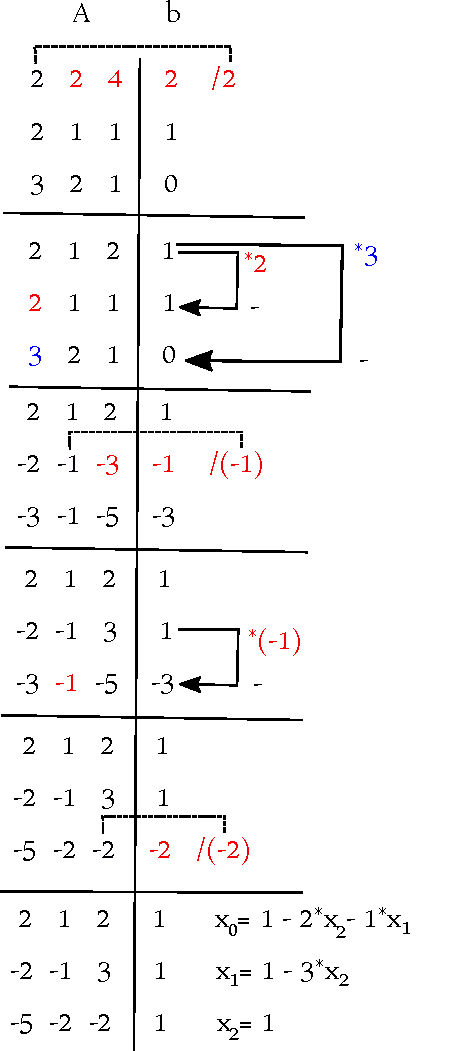
\includegraphics{graph.pdf}
    \caption{Demonstration of Gaussian Elimination}
    \label{graph}
  \end{center}
\end{figure}

\subsubsection*{Solving a linear system of rank 3 cannot be vectorized efficiently. Explain why.}
The algorithm implemented in gauss.c has several read-after-write conflicts. For instance, when dividing entries in the first row of A by $a_{00}$, $a_{01}$ is overwritten. Upon updating the second row, $a_{01}$ is read. Entries from the second row are again read when updating the third row. For $n$ higher than 3, it is possible that there are enough operations between conflicting ones to allow for optimal vectorization.
\section{Matrix-Matrix-Multiplication I}

\subsection*{Examine the memory access of the given implementation.}

The accessed memory location of \texttt{c} is constant within the innermost loop. Access to \texttt{a} is with unit-stride, access to \texttt{b} is with stride n.

\subsection*{Use different compiler-directives (Intel compiler) in order to vectorize the given code.}

Compiling with the option \texttt{-O3} enables auto-vectorization and high-level optimizations using advanced loop transformations.

The only thing that could be done in order to support auto-vectorization is to allocate the arrays with \texttt{memalign()} instead of the default \texttt{malloc()} function and provide the compiler with the hint \texttt{\#pragma vector aligned} just before the innermost loop. Otherwise there is no need for additional compiler directives.

\subsection*{Measure MFLOPS rates and cache-miss-rates for different problems sizes and plot your results. Please use Valgrind for measuring the cache-miss rate.}

Sample data was recorded using the modified program \texttt{dgemm\_variable\_problem\_size.c} and the shell script \texttt{collect\_data1.sh}.

\subsection*{Do different compiler options (please use the compiler manual for more aggressive options) influence the performance of the implementation.}

Yes. Without optimizations (\texttt{-O0}) the are roughly ten times less FLOPS (compared to \texttt{-O3}). With basic optimizations (\texttt{-O1}) things improve roughly by a factor of three (compared to \texttt{-O0}) and with vectorization (\texttt{-O2}) by a factor of ten. High-level optimizations (\texttt{-O3}) don't improve things anymore compare to \texttt{-O2}.

Using the preset \texttt{-fast} improves the performance slightly by a factor of roughly 1.5 compared to \texttt{-O3}. It effectively worsens the precision of floating point arithmetic and links runtime dependencies statically.

\subsection*{For which problem size do you get the best performance?}

\subsection*{Is the obtained performance stable?}

\subsection*{Please explain the obtained performance using hardware properties (such as cache size, memory bandwidth, or similar).}

\end{document}
